% !TeX spellcheck = en_US
\chapter{Graphical Models}

For more examples, exercises with solutions, check:
\begin{itemize}
	\item \citeaustitle{bishop2006pattern}
\end{itemize}

\section{Bayesian Network}
Bayesian networks, \ac{aka}, Bayes nets, Belief networks and sometimes Causal networks, are graphical representation of a probabilistic model. It comprises of nodes and directed edges.
\begin{itemize}
	\item Nodes represent variable (continuous or discrete)
	\item Edges represent dependency between variables
\end{itemize}

\begin{figure}[hbt!]
	\centering
	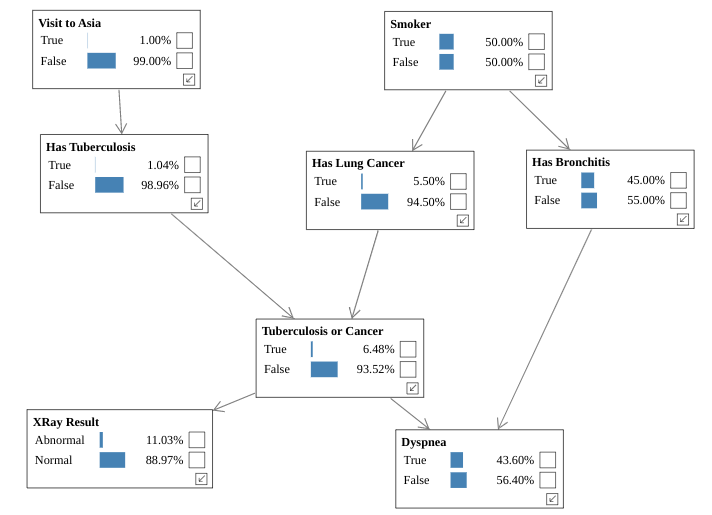
\includegraphics[width=0.7\textwidth]{bayesian-asia-network.png}
	\caption{Example of Bayesian network: the Asia network (\href{https://www.bayesserver.com/examples/networks/asia}{src}).}
	\label{fig:bayesian-asia-network}
\end{figure}

They are useful in a variety of tasks
\begin{itemize}
	\item Descriptive analytic
	\item Diagnostic analytic
	\item Predictive analytic
	\item Prescriptive analytic
\end{itemize}